% 若编译失败,且生成 .synctex(busy) 辅助文件,可能有两个原因:
% 1. 需要插入的图片不存在:Ctrl + F 搜索 'figure' 将这些代码注释/删除掉即可
% 2. 路径/文件名含中文或空格:更改路径/文件名即可

% ------------------------------------------------------------- %
% >> ------------------ 文章宏包及相关设置 ------------------ << %
% 设定文章类型与编码格式
\documentclass[UTF8]{report}		

% 本文特殊宏包
\usepackage{siunitx} % 埃米单位

% 本 .tex 专属的宏定义
    \def\V{\ \mathrm{V}}
    \def\mV{\ \mathrm{mV}}
    \def\kV{\ \mathrm{KV}}
    \def\KV{\ \mathrm{KV}}
    \def\MV{\ \mathrm{MV}}
    \def\A{\ \mathrm{A}}
    \def\mA{\ \mathrm{mA}}
    \def\kA{\ \mathrm{KA}}
    \def\KA{\ \mathrm{KA}}
    \def\MA{\ \mathrm{MA}}
    \def\O{\ \Omega}
    \def\mO{\ \Omega}
    \def\kO{\ \mathrm{K}\Omega}
    \def\KO{\ \mathrm{K}\Omega}
    \def\MO{\ \mathrm{M}\Omega}
    \def\Hz{\ \mathrm{Hz}}

% 自定义宏定义
    \def\N{\mathbb{N}}
    \def\F{\mathbb{F}}
    \def\Z{\mathbb{Z}}
    \def\Q{\mathbb{Q}}
    \def\R{\mathbb{R}}
    \def\C{\mathbb{C}}
    \def\T{\mathbb{T}}
    \def\S{\mathbb{S}}
    \def\A{\mathbb{A}}
    \def\I{\mathscr{I}}
    \def\Im{\mathrm{Im\,}}
    \def\Re{\mathrm{Re\,}}
    \def\d{\mathrm{d}}
    \def\p{\partial}

% 导入基本宏包
    \usepackage[UTF8]{ctex}     % 设置文档为中文语言
    \usepackage[colorlinks, linkcolor=blue, anchorcolor=blue, citecolor=blue, urlcolor=blue]{hyperref}  % 宏包:自动生成超链接 (此宏包与标题中的数学环境冲突)
    % \usepackage{hyperref}  % 宏包:自动生成超链接 (此宏包与标题中的数学环境冲突)
    % \hypersetup{
    %     colorlinks=true,    % false:边框链接 ; true:彩色链接
    %     citecolor={blue},    % 文献引用颜色
    %     linkcolor={blue},   % 目录 (我们在目录处单独设置),公式,图表,脚注等内部链接颜色
    %     urlcolor={orange},    % 网页 URL 链接颜色,包括 \href 中的 text
    %     % cyan 浅蓝色 
    %     % magenta 洋红色
    %     % yellow 黄色
    %     % black 黑色
    %     % white 白色
    %     % red 红色
    %     % green 绿色
    %     % blue 蓝色
    %     % gray 灰色
    %     % darkgray 深灰色
    %     % lightgray 浅灰色
    %     % brown 棕色
    %     % lime 石灰色
    %     % olive 橄榄色
    %     % orange 橙色
    %     % pink 粉红色
    %     % purple 紫色
    %     % teal 蓝绿色
    %     % violet 紫罗兰色
    % }

    % \usepackage{docmute}    % 宏包:子文件导入时自动去除导言区,用于主/子文件的写作方式,\include{./51单片机笔记}即可。注:启用此宏包会导致.tex文件capacity受限。
    \usepackage{amsmath}    % 宏包:数学公式
    \usepackage{mathrsfs}   % 宏包:提供更多数学符号
    \usepackage{amssymb}    % 宏包:提供更多数学符号
    \usepackage{pifont}     % 宏包:提供了特殊符号和字体
    \usepackage{extarrows}  % 宏包:更多箭头符号
    \usepackage{multicol}   % 宏包:支持多栏 
    \usepackage{graphicx}   % 宏包:插入图片
    \usepackage{float}      % 宏包:设置图片浮动位置
    %\usepackage{article}    % 宏包:使文本排版更加优美
    \usepackage{tikz}       % 宏包:绘图工具
    %\usepackage{pgfplots}   % 宏包:绘图工具
    \usepackage{enumerate}  % 宏包:列表环境设置
    \usepackage{enumitem}   % 宏包:列表环境设置
    \usepackage[all]{xy} % 宏包:xy图形
    \usepackage{tikz-cd} % 宏包:xy图形

% 文章页面margin设置
    \usepackage[a4paper]{geometry}
        \geometry{top=1in}
        \geometry{bottom=1in}
        \geometry{left=0.75in}
        \geometry{right=0.75in}   % 设置上下左右页边距
        \geometry{marginparwidth=1.75cm}    % 设置边注距离(注释、标记等)

% 定义 solution 环境
\usepackage{amsthm}
\newtheorem{solution}{Solution}
        \geometry{bottom=1in}
        \geometry{left=0.75in}
        \geometry{right=0.75in}   % 设置上下左右页边距
        \geometry{marginparwidth=1.75cm}    % 设置边注距离(注释、标记等)

% 配置数学环境
    \usepackage{amsthm} % 宏包:数学环境配置
    % theorem-line 环境自定义
        \newtheoremstyle{MyLineTheoremStyle}% <name>
            {11pt}% <space above>
            {11pt}% <space below>
            {}% <body font> 使用默认正文字体
            {}% <indent amount>
            {\bfseries}% <theorem head font> 设置标题项为加粗
            {:}% <punctuation after theorem head>
            {.5em}% <space after theorem head>
            {\textbf{#1}\thmnumber{#2}\ \ (\,\textbf{#3}\,)}% 设置标题内容顺序
        \theoremstyle{MyLineTheoremStyle} % 应用自定义的定理样式
        \newtheorem{LineTheorem}{Theorem.\,}
    % theorem-block 环境自定义
        \newtheoremstyle{MyBlockTheoremStyle}% <name>
            {11pt}% <space above>
            {11pt}% <space below>
            {}% <body font> 使用默认正文字体
            {}% <indent amount>
            {\bfseries}% <theorem head font> 设置标题项为加粗
            {:\\ \indent}% <punctuation after theorem head>
            {.5em}% <space after theorem head>
            {\textbf{#1}\thmnumber{#2}\ \ (\,\textbf{#3}\,)}% 设置标题内容顺序
        \theoremstyle{MyBlockTheoremStyle} % 应用自定义的定理样式
        \newtheorem{BlockTheorem}[LineTheorem]{Theorem.\,} % 使用 LineTheorem 的计数器
    % definition 环境自定义
        \newtheoremstyle{MySubsubsectionStyle}% <name>
            {11pt}% <space above>
            {11pt}% <space below>
            {}% <body font> 使用默认正文字体
            {}% <indent amount>
            {\bfseries}% <theorem head font> 设置标题项为加粗
           % {:\\ \indent}% <punctuation after theorem head>
            {\\\indent}
            {0pt}% <space after theorem head>
            {\textbf{#3}}% 设置标题内容顺序
        \theoremstyle{MySubsubsectionStyle} % 应用自定义的定理样式
        \newtheorem{definition}{}

%宏包:有色文本框(proof环境)及其设置
    \usepackage[dvipsnames,svgnames]{xcolor}    %设置插入的文本框颜色
    \usepackage[strict]{changepage}     % 提供一个 adjustwidth 环境
    \usepackage{framed}     % 实现方框效果
        \definecolor{graybox_color}{rgb}{0.95,0.95,0.96} % 文本框颜色。修改此行中的 rgb 数值即可改变方框纹颜色,具体颜色的rgb数值可以在网站https://colordrop.io/ 中获得。(截止目前的尝试还没有成功过,感觉单位不一样)(找到喜欢的颜色,点击下方的小眼睛,找到rgb值,复制修改即可)
        \newenvironment{graybox}{%
        \def\FrameCommand{%
        \hspace{1pt}%
        {\color{gray}\small \vrule width 2pt}%
        {\color{graybox_color}\vrule width 4pt}%
        \colorbox{graybox_color}%
        }%
        \MakeFramed{\advance\hsize-\width\FrameRestore}%
        \noindent\hspace{-4.55pt}% disable indenting first paragraph
        \begin{adjustwidth}{}{7pt}%
        \vspace{2pt}\vspace{2pt}%
        }
        {%
        \vspace{2pt}\end{adjustwidth}\endMakeFramed%
        }



% 外源代码插入设置
    % matlab 代码插入设置
    \usepackage{matlab-prettifier}
        \lstset{style=Matlab-editor}    % 继承 matlab 代码高亮 , 此行不能删去
    \usepackage[most]{tcolorbox} % 引入tcolorbox包 
    \usepackage{listings} % 引入listings包
        \tcbuselibrary{listings, skins, breakable}
        \newfontfamily\codefont{Consolas} % 定义需要的 codefont 字体
        \lstdefinestyle{MatlabStyle_inc}{   % 插入代码的样式
            language=Matlab,
            basicstyle=\small\ttfamily\codefont,    % ttfamily 确保等宽 
            breakatwhitespace=false,
            breaklines=true,
            captionpos=b,
            keepspaces=true,
            numbers=left,
            numbersep=15pt,
            showspaces=false,
            showstringspaces=false,
            showtabs=false,
            tabsize=2,
            xleftmargin=15pt,   % 左边距
            %frame=single, % single 为包围式单线框
            frame=shadowbox,    % shadowbox 为带阴影包围式单线框效果
            %escapeinside=``,   % 允许在代码块中使用 LaTeX 命令 (此行无用)
            %frameround=tttt,    % tttt 表示四个角都是圆角
            framextopmargin=0pt,    % 边框上边距
            framexbottommargin=0pt, % 边框下边距
            framexleftmargin=5pt,   % 边框左边距
            framexrightmargin=5pt,  % 边框右边距
            rulesepcolor=\color{red!20!green!20!blue!20}, % 阴影框颜色设置
            %backgroundcolor=\color{blue!10}, % 背景颜色
        }
        \lstdefinestyle{MatlabStyle_src}{   % 插入代码的样式
            language=Matlab,
            basicstyle=\small\ttfamily\codefont,    % ttfamily 确保等宽 
            breakatwhitespace=false,
            breaklines=true,
            captionpos=b,
            keepspaces=true,
            numbers=left,
            numbersep=15pt,
            showspaces=false,
            showstringspaces=false,
            showtabs=false,
            tabsize=2,
        }
        \newtcblisting{matlablisting}{
            %arc=2pt,        % 圆角半径
            % 调整代码在 listing 中的位置以和引入文件时的格式相同
            top=0pt,
            bottom=0pt,
            left=-5pt,
            right=-5pt,
            listing only,   % 此句不能删去
            listing style=MatlabStyle_src,
            breakable,
            colback=white,   % 选一个合适的颜色
            colframe=black!0,   % 感叹号后跟不透明度 (为 0 时完全透明)
        }
        \lstset{
            style=MatlabStyle_inc,
        }



% table 支持
    \usepackage{booktabs}   % 宏包:三线表
    %\usepackage{tabularray} % 宏包:表格排版
    %\usepackage{longtable}  % 宏包:长表格
    %\usepackage[longtable]{multirow} % 宏包:multi 行列


% figure 设置
\usepackage{graphicx}   % 支持 jpg, png, eps, pdf 图片 
\usepackage{float}      % 支持 H 选项
\usepackage{svg}        % 支持 svg 图片
\usepackage{subcaption} % 支持子图
\svgsetup{
        % 指向 inkscape.exe 的路径
       inkscapeexe = C:/aa_MySame/inkscape/bin/inkscape.exe, 
        % 一定程度上修复导入后图片文字溢出几何图形的问题
       inkscapelatex = false                 
   }

% 图表进阶设置
    \usepackage{caption}    % 图注、表注
        \captionsetup[figure]{name=图}  
        \captionsetup[table]{name=表}
        \captionsetup{
            labelfont=bf, % 设置标签为粗体
            textfont=bf,  % 设置文本为粗体
            font=small  
        }
    \usepackage{float}     % 图表位置浮动设置 
        % \floatstyle{plaintop} % 设置表格标题在表格上方
        % \restylefloat{table}  % 应用设置


% 圆圈序号自定义
    \newcommand*\circled[1]{\tikz[baseline=(char.base)]{\node[shape=circle,draw,inner sep=0.8pt, line width = 0.03em] (char) {\small \bfseries #1};}}   % TikZ solution


% 列表设置
    \usepackage{enumitem}   % 宏包:列表环境设置
        \setlist[enumerate]{
            label=\bfseries(\arabic*) ,   % 设置序号样式为加粗的 (1) (2) (3)
            ref=\arabic*, % 如果需要引用列表项,这将决定引用格式(这里仍然使用数字)
            itemsep=0pt, parsep=0pt, topsep=0pt, partopsep=0pt, leftmargin=3.5em} 
        \setlist[itemize]{itemsep=0pt, parsep=0pt, topsep=0pt, partopsep=0pt, leftmargin=3.5em}
        \newlist{circledenum}{enumerate}{1} % 创建一个新的枚举环境  
        \setlist[circledenum,1]{  
            label=\protect\circled{\arabic*}, % 使用 \arabic* 来获取当前枚举计数器的值,并用 \circled 包装它  
            ref=\arabic*, % 如果需要引用列表项,这将决定引用格式(这里仍然使用数字)
            itemsep=0pt, parsep=0pt, topsep=0pt, partopsep=0pt, leftmargin=3.5em
        }  

% 文章默认字体设置
    \usepackage{fontspec}   % 宏包:字体设置
        \setmainfont{STKaiti}    % 设置中文字体为宋体字体
        \setCJKmainfont[AutoFakeBold=3]{STKaiti} % 设置加粗字体为 STKaiti 族,AutoFakeBold 可以调整字体粗细
        \setmainfont{Times New Roman} % 设置英文字体为Times New Roman


% 其它设置
    % 脚注设置
    \renewcommand\thefootnote{\ding{\numexpr171+\value{footnote}}}
    % 参考文献引用设置
        \bibliographystyle{unsrt}   % 设置参考文献引用格式为unsrt
        \newcommand{\upcite}[1]{\textsuperscript{\cite{#1}}}     % 自定义上角标式引用
    % 文章序言设置
        \newcommand{\cnabstractname}{序言}
        \newenvironment{cnabstract}{%
            \par\Large
            \noindent\mbox{}\hfill{\bfseries \cnabstractname}\hfill\mbox{}\par
            \vskip 2.5ex
            }{\par\vskip 2.5ex}


% 各级标题自定义设置
    \usepackage{titlesec}   
    % chapter
        \titleformat{\chapter}[hang]{\normalfont\Large\bfseries\centering}{Chapter \thechapter }{10pt}{}
        \titlespacing*{\chapter}{0pt}{-30pt}{10pt} % 控制上方空白的大小
    % section
        \titleformat{\section}[hang]{\normalfont\large\bfseries}{\thesection}{8pt}{}
    % subsection
        %\titleformat{\subsubsection}[hang]{\normalfont\bfseries}{}{8pt}{}
    % subsubsection
        %\titleformat{\subsubsection}[hang]{\normalfont\bfseries}{}{8pt}{}

% 见到的一个有意思的对于公式中符号的彩色解释的环境
        \usepackage[dvipsnames]{xcolor}
        \usepackage{tikz}
        \usetikzlibrary{backgrounds}
        \usetikzlibrary{arrows,shapes}
        \usetikzlibrary{tikzmark}
        \usetikzlibrary{calc}
        
        \usepackage{amsmath}
        \usepackage{amsthm}
        \usepackage{amssymb}
        \usepackage{mathtools, nccmath}
        \usepackage{wrapfig}
        \usepackage{comment}
        
        % To generate dummy text
        \usepackage{blindtext}
        
        
        %color
        %\usepackage[dvipsnames]{xcolor}
        % \usepackage{xcolor}
        
        
        %\usepackage[pdftex]{graphicx}
        \usepackage{graphicx}
        % declare the path(s) for graphic files
        %\graphicspath{{../Figures/}}
        
        % extensions so you won't have to specify these with
        % every instance of \includegraphics
        % \DeclareGraphicsExtensions{.pdf,.jpeg,.png}
        
        % for custom commands
        \usepackage{xspace}
        
        % table alignment
        \usepackage{array}
        \usepackage{ragged2e}
        \newcolumntype{P}[1]{>{\RaggedRight\hspace{0pt}}p{#1}}
        \newcolumntype{X}[1]{>{\RaggedRight\hspace*{0pt}}p{#1}}
        
        % color box
        \usepackage{tcolorbox}
        
        
        % for tikz
        \usepackage{tikz}
        %\usetikzlibrary{trees}
        \usetikzlibrary{arrows,shapes,positioning,shadows,trees,mindmap}
        % \usepackage{forest}
        \usepackage[edges]{forest}
        \usetikzlibrary{arrows.meta}
        \colorlet{linecol}{black!75}
        \usepackage{xkcdcolors} % xkcd colors
        
        
        % for colorful equation
        \usepackage{tikz}
        \usetikzlibrary{backgrounds}
        \usetikzlibrary{arrows,shapes}
        \usetikzlibrary{tikzmark}
        \usetikzlibrary{calc}
        % Commands for Highlighting text -- non tikz method
        \newcommand{\highlight}[2]{\colorbox{#1!17}{$\displaystyle #2$}}
        %\newcommand{\highlight}[2]{\colorbox{#1!17}{$#2$}}
        \newcommand{\highlightdark}[2]{\colorbox{#1!47}{$\displaystyle #2$}}
        
        % my custom colors for shading
        \colorlet{mhpurple}{Plum!80}
        
        
        % Commands for Highlighting text -- non tikz method
        \renewcommand{\highlight}[2]{\colorbox{#1!17}{#2}}
        \renewcommand{\highlightdark}[2]{\colorbox{#1!47}{#2}}
        
        % Some math definitions
        \newcommand{\lap}{\mathrm{Lap}}
        \newcommand{\pr}{\mathrm{Pr}}
        
        \newcommand{\Tset}{\mathcal{T}}
        \newcommand{\Dset}{\mathcal{D}}
        \newcommand{\Rbound}{\widetilde{\mathcal{R}}}

% >> ------------------ 文章宏包及相关设置 ------------------ << %
% ------------------------------------------------------------- %



% ----------------------------------------------------------- %
% >> --------------------- 文章信息区 --------------------- << %
% 页眉页脚设置

\usepackage{fancyhdr}   %宏包:页眉页脚设置
    \pagestyle{fancy}
    \fancyhf{}
    \cfoot{\thepage}
    \renewcommand\headrulewidth{1pt}
    \renewcommand\footrulewidth{0pt}
    \chead{尹超,\ 工号:BGI39771}
    \lhead{华大基因实习总结}
    \rhead{yinchao23@mails.ucas.ac.cn}

%文档信息设置
\title{华大基因实习总结\\ BGI Genomics Internship Summary}
\author{尹超\\ \footnotesize 中国科学院大学,北京 100049\\ Carter Yin \\ \footnotesize University of Chinese Academy of Sciences, Beijing 100049, China}
\date{\footnotesize 2025.7.21 -- 2025.8.22}
% >> --------------------- 文章信息区 --------------------- << %
% ----------------------------------------------------------- %     


% 开始编辑文章

\begin{document}
\zihao{5}           % 设置全文字号大小

% --------------------------------------------------------------- %
% >> --------------------- 封面序言与目录 --------------------- << %
% 封面
    \maketitle\newpage  
    \pagenumbering{Roman} % 页码为大写罗马数字
    \thispagestyle{fancy}   % 显示页码、页眉等

% 序言
    \begin{cnabstract}\normalsize 
        本文为笔者在华大基因实习期间的工作总结。\par
        望师兄师姐批评指正。
    \end{cnabstract}
    \addcontentsline{toc}{chapter}{序言} % 手动添加为目录

% % 不换页目录
%     \setcounter{tocdepth}{0}
%     \noindent\rule{\textwidth}{0.1em}   % 分割线
%     \noindent\begin{minipage}{\textwidth}\centering 
%         \vspace{1cm}
%         \tableofcontents\thispagestyle{fancy}   % 显示页码、页眉等   
%     \end{minipage}  
%     \addcontentsline{toc}{chapter}{目录} % 手动添加为目录

% 目录
\setcounter{tocdepth}{4}                % 目录深度(为1时显示到section)
\tableofcontents                        % 目录页
\addcontentsline{toc}{chapter}{目录}    % 手动添加此页为目录
\thispagestyle{fancy}                   % 显示页码、页眉等 

% 收尾工作
    \newpage    
    \pagenumbering{arabic} 

% >> --------------------- 封面序言与目录 --------------------- << %
% --------------------------------------------------------------- %


\chapter{工作材料}

\section{数据分析:chart文件夹}

该文件夹主要包含数据分析过程中生成的可视化图表和代码,具体包括:

\textbf{数据与代码文件}
\begin{itemize}
    \item \texttt{analysis\_result\_eyes\_realigned.tsv}绘图数据文件
    \item \texttt{disease\_groups\_histogram.py}:绘制眼病患病率和其他疾病患病率的样本数量分布。
    \item \texttt{disease\_groups\_histogram2.py}:绘制其他疾病患病率的样本数量分布。
    \item \texttt{exclude\_max\_histogram.py}:剔除最大值后绘制样本数量分布。
    \item \texttt{max\_vs\_others\_histogram.py}:绘制最大值与其他值的样本数量分布。
\end{itemize}

\textbf{图片文件}
\begin{itemize}
    \item \texttt{eye\_diseases\_bar.png}
    \item \texttt{other\_diseases\_bar.png}
    \item \texttt{other\_diseases\_bar\_new.png}
    \item \texttt{exclude\_max\_histogram\_ultra\_high.png}
    \item \texttt{max\_vs\_others\_histogram\_ultra\_high.png}
\end{itemize}



\section{原始数据文件修正:pre\_mod文件夹}

\subsection{代码与数据文件}
data\_preprocessing.py

original.tsv

\subsection{代码实现}

\begin{itemize}
    \item \texttt{data\_preprocessing.py}:该脚本的具体实现步骤如下:
    \begin{enumerate}
        \item 读取输入的original.tsv文件。
        \item 对原始数据文件进行添加列标题samples,为保证tsv文件列对齐。
        \item 遍历数据,将除了第一列的样本编号外的“yes”替换为1。
        \item 遍历数据,将除了第一列的样本编号外的“no”替换为0。
        \item 将处理后的数据写入新的preprocessing.tsv文件中。
    \end{enumerate}
    \item \texttt{preprocessing.tsv}:该文件为经过处理后的tsv文件。
    \item \texttt{original.tsv.original\_backup}:该文件为原始数据文件的备份。
\end{itemize}


\section{数据预处理:backup文件夹}

在数据分析之前,首先需要对原始数据进行预处理。数据预处理的主要步骤包括:(其中Step6为了结构完整性保留在此,仅为提及)

\begin{itemize}
    \item[Step 0:] 剔除没有疾病诊断信息的个体(青光眼,黄斑变性,白内障,糖尿病,中风,高血压,缺血性心脏病)
    \item[Step 1:] 剔除眼病患者(青光眼,黄斑变性,白内障),用作test (剩余21137 samples)
    \item[Step 2:] 剔除其它有记录的疾病患者(糖尿病,中风,高血压,缺血性心脏病),用作test (剩余11895 samples)
    \item[Step 3:] 删去方差为0的列,并将数据集分为training set(80\%)和test set(20\%)
    \item[Step 4:] 针对training 和test内的数据缺失分别进行补全(剔除缺失率过高的字段),这里我们采用了Mean imputation
    \item[Step 5:] 筛选字段 – v3眼部字段,颈动脉字段,生理代谢字段
    \item[Step 6:] 基于不同的数据组合,如眼部数据、颈动脉数据、生理数据和所有数据,计算生物学年龄,训练基于决策树类算法的预测模型,包括XGBoost, LightGBM, CatBoost,Random Forest。
\end{itemize}

\subsection*{Step 0}
\addcontentsline{toc}{subsection}{Step 0}

\textbf{step0.py}:该脚本的主要功能是剔除没有疾病诊断信息的个体。具体实现步骤如下:
\begin{enumerate}
    \item 读取输入的tsv文件。
    \item 遍历数据,对于指定的字段,如果全为NA,则剔除该个体。
    \item 将处理后的数据写入新的tsv文件中。
\end{enumerate}

\subsection*{Step 1}
\addcontentsline{toc}{subsection}{Step 1}

\textbf{step1.py}:该脚本的主要功能是剔除眼病患者。具体实现步骤如下:
\begin{enumerate}
    \item 读取输入的tsv文件。
    \item 遍历数据,对于指定的眼科疾病诊断字段,如果值为1,则剔除该个体。
    \item 将处理后的数据写入新的tsv文件中。
\end{enumerate}

\subsection*{Step 2}
\addcontentsline{toc}{subsection}{Step 2}

\textbf{step2.py}:该脚本的主要功能是剔除其它有记录的疾病患者。具体实现步骤如下:
\begin{enumerate}
    \item 读取输入的tsv文件。
    \item 遍历数据,对于指定的其它疾病诊断字段,如果值为1,则剔除该个体。
    \item 将处理后的数据写入新的tsv文件中。
\end{enumerate}

\subsection*{Step 3}
\addcontentsline{toc}{subsection}{Step 3}

\textbf{step3.py}:该脚本的主要功能是删去方差为0的列,并将数据集分为训练集和测试集。具体实现步骤如下:
\begin{enumerate}
    \item 读取输入的tsv文件。
    \item 删去方差为0的列。
    \item 随机打乱数据顺序。
    \item 按照8:2的比例划分训练集和测试集。
    \item 将训练集和测试集分别写入新的tsv文件中。
\end{enumerate}


\subsection*{Step 4}
\addcontentsline{toc}{subsection}{Step 4}

\textbf{step4.py}:该脚本的主要功能如下:
\begin{enumerate}
    \item 读取输入的tsv文件。
    \item 遍历数据,对于缺失值超过50\%的字段,剔除该字段。
    \item 遍历数据,对于缺失的特定字段值,按照优先级规则进行填充。
    \item 仅保留指定的124个字段。
    \item 遍历数据,对于缺失的其它字段值,按照填充规则进行填充。
    \item 将处理后的数据写入新的tsv文件中。
\end{enumerate}

\begin{center}
\fbox{
    \begin{minipage}{0.95\textwidth}
    \textbf{特定字段填充规则:}
    \begin{enumerate}
        \item \textbf{bmi\_x10}:如果为空,使用 \texttt{bmi\_calc\_resurvey2} $\times$ 10 或 \texttt{bmi\_calc\_baseline} $\times$ 10 填充\\
        \quad 优先级:\texttt{bmi\_calc\_resurvey2} $>$ \texttt{bmi\_calc\_baseline}
        \item \textbf{standing\_height\_cm\_x10}:如果为空,使用 \texttt{standing\_height\_mm\_resurvey2} 或 \texttt{standing\_height\_mm\_baseline} 填充\\
        \quad 优先级:\texttt{standing\_height\_mm\_resurvey2} $>$ \texttt{standing\_height\_mm\_baseline}
        \item \textbf{weight\_kg\_x10\_resurvey3}:如果为空,使用 \texttt{weight\_kg\_x10\_resurvey2} 或 \texttt{weight\_kg\_x10\_baseline} 填充\\
        \quad 优先级:\texttt{weight\_kg\_x10\_resurvey2} $>$ \texttt{weight\_kg\_x10\_baseline}
    \end{enumerate}
    \end{minipage}
}
\end{center}

\begin{center}
\fbox{
    \begin{minipage}{0.95\textwidth}
    \textbf{其它填充规则:}
    \begin{enumerate}
        \item 如果列只包含少数几个值(≤10个唯一值),按照填充前的比例进行随机填充
        \item 对于 \texttt{id\_ethnic\_group\_id} 这一列,按照情况1处理
        \item 如果是其他情况,按照均值填充缺失值
    \end{enumerate}
    \end{minipage}
}
\end{center}

\subsection*{Step 5\_0base}
\addcontentsline{toc}{subsection}{Step 5\_0base}

\textbf{该文件夹存放了整个步骤5中的基础数据文件。}\par


\subsection*{Step 5\_1eye}
\addcontentsline{toc}{subsection}{Step 5\_1eye}

\textbf{eye.py}:该脚本的主要功能是筛选眼科相关字段。具体实现步骤如下:
\begin{enumerate}
    \item 读取输入的tsv文件。
    \item 仅保留与眼科相关的字段。
    \item 将处理后的数据写入新的tsv文件中。
\end{enumerate}

\subsection*{Step 5\_2artery}
\addcontentsline{toc}{subsection}{Step 5\_2artery}

\textbf{artery.py}:该脚本的主要功能是筛选动脉相关字段。具体实现步骤如下:
\begin{enumerate}
    \item 读取输入的tsv文件。
    \item 仅保留与动脉相关的字段。
    \item 将处理后的数据写入新的tsv文件中。
\end{enumerate} 

\subsection*{Step 5\_3physiology}
\addcontentsline{toc}{subsection}{Step 5\_3physiology}

\textbf{physiology.py}:该脚本的主要功能是筛选生理相关字段。具体实现步骤如下:
\begin{enumerate}
    \item 读取输入的tsv文件。
    \item 仅保留与生理相关的字段。(不包括年龄)
    \item 将处理后的数据写入新的tsv文件中。
\end{enumerate}

\subsection*{Step 5\_4all}
\addcontentsline{toc}{subsection}{Step 5\_4all}

\textbf{all.py}:该脚本的主要功能是筛选所有指定字段。具体实现步骤如下:
\begin{enumerate}
    \item 读取输入的tsv文件。
    \item 保留所有指定字段。(不包括年龄)
    \item 将处理后的数据写入新的tsv文件中。
\end{enumerate}


\subsection*{Step 5\_5age}
\addcontentsline{toc}{subsection}{Step 5\_5age}

\textbf{age.py}:该脚本的主要功能是筛选年龄相关字段。具体实现步骤如下:
\begin{enumerate}
    \item 读取输入的tsv文件。
    \item 仅保留与年龄相关的字段。
    \item 将处理后的数据写入新的tsv文件中。
\end{enumerate}


\subsection*{Step 5\_6ren}
\addcontentsline{toc}{subsection}{Step 5\_6ren}

\textbf{ren.py}:该脚本的主要功能是筛选人口学相关字段。具体实现步骤如下:
\begin{enumerate}
    \item 读取输入的tsv文件。
    \item 仅保留与性别、地区和职业相关的字段。
    \item 将处理后的数据写入新的tsv文件中。
\end{enumerate}

\subsection*{Step 5\_7newall}
\addcontentsline{toc}{subsection}{Step 5\_7newall}

\textbf{newall.py}:该脚本的主要功能是合并新增的人口学指标和原来指定的所有字段。具体实现步骤如下:
\begin{enumerate}
    \item 读取输入的tsv文件。
    \item 合并新增的人口学指标和原来指定的所有字段。
    \item 将处理后的数据写入新的tsv文件中。
\end{enumerate}




\section{模型训练和测试:train\_test文件夹}
\textbf{使用不同的数据预测生物学年龄}\par
\textbf{该文件夹下的所有子文件夹的结构如下:}

\begin{center}
\begin{verbatim}
train_test/all/
|-- code/
|   |-- catboost_info/
|   |   |-- learn/
|   |   |-- tmp/
|   |   |-- catboost_training.json
|   |   |-- learn_error.tsv
|   |   |-- time_left.tsv
|   |-- __pycache__/
|   |-- hyperparameter_tuning_gpu_report.txt
|   |-- simple1_gpu.py
|-- train_all.tsv
|-- test_all.tsv
|-- train_age.tsv
|-- test_age.tsv
\end{verbatim}
\end{center}

\subsection*{all}
\addcontentsline{toc}{subsection}{all}

\textbf{simple1\_gpu.py}:该脚本的主要功能是对所有数据进行模型训练和测试。具体实现步骤如下:
\begin{enumerate}
    \item 读取输入的tsv文件。
    \item 对数据进行预处理,包括去除缺失值、标准化等。
    \item 校正项计算函数。
    \item 在四种不同的模型上进行训练。(XGBoost, LightGBM, CatBoost, RandomForest)
    \item 训练集上进行五折交叉验证寻找最佳超参数。(以MAE为指标)
    \item 在测试集上分别评估四种模型最佳参数的性能。
    \item 输出报告。
\end{enumerate}

\subsection*{artery}
\addcontentsline{toc}{subsection}{artery}

\textbf{simple1\_gpu.py}:该脚本的主要功能是对颈动脉数据进行模型训练和测试。具体实现步骤如下:
\begin{enumerate}
    \item 读取输入的tsv文件。
    \item 对数据进行预处理,包括去除缺失值、标准化等。
    \item 校正项计算函数。
    \item 在四种不同的模型上进行训练。(XGBoost, LightGBM, CatBoost, RandomForest)
    \item 训练集上进行五折交叉验证寻找最佳超参数。(以MAE为指标)
    \item 在测试集上分别评估四种模型最佳参数的性能。
    \item 输出报告。
\end{enumerate}

\subsection*{eye}
\addcontentsline{toc}{subsection}{eye}

\textbf{simple1\_gpu.py}:该脚本的主要功能是对眼科数据进行模型训练和测试。具体实现步骤如下:
\begin{enumerate}
    \item 读取输入的tsv文件。
    \item 对数据进行预处理,包括去除缺失值、标准化等。
    \item 校正项计算函数。
    \item 在四种不同的模型上进行训练。(XGBoost, LightGBM, CatBoost, RandomForest)
    \item 训练集上进行五折交叉验证寻找最佳超参数。(以MAE为指标)
    \item 在测试集上分别评估四种模型最佳参数的性能。
    \item 输出报告。
\end{enumerate}

\subsection*{physiology}
\addcontentsline{toc}{subsection}{physiology}

\textbf{simple1\_gpu.py}:该脚本的主要功能是对生理数据进行模型训练和测试。具体实现步骤如下:
\begin{enumerate}
    \item 读取输入的tsv文件。
    \item 对数据进行预处理,包括去除缺失值、标准化等。
    \item 校正项计算函数。
    \item 在四种不同的模型上进行训练。(XGBoost, LightGBM, CatBoost, RandomForest)
    \item 训练集上进行五折交叉验证寻找最佳超参数。(以MAE为指标)
    \item 在测试集上分别评估四种模型最佳参数的性能。
    \item 输出报告。
\end{enumerate}

\subsection*{ren}
\addcontentsline{toc}{subsection}{ren}

\textbf{simple1\_gpu.py}:该脚本的主要功能是对人口学数据进行模型训练和测试。具体实现步骤如下:
\begin{enumerate}
    \item 读取输入的tsv文件。
    \item 对数据进行预处理,包括去除缺失值、标准化等。
    \item 校正项计算函数。
    \item 在四种不同的模型上进行训练。(XGBoost, LightGBM, CatBoost, RandomForest)
    \item 训练集上进行五折交叉验证寻找最佳超参数。(以MAE为指标)
    \item 在测试集上分别评估四种模型最佳参数的性能。
    \item 输出报告。
\end{enumerate}


\subsection*{newall}
\addcontentsline{toc}{subsection}{newall}

\textbf{simple1\_gpu.py}:该脚本的主要功能是对新的所有数据(新增了人口学数据)进行模型训练和测试。具体实现步骤如下:
\begin{enumerate}
    \item 读取输入的tsv文件。
    \item 对数据进行预处理,包括去除缺失值、标准化等。
    \item 校正项计算函数。
    \item 在四种不同的模型上进行训练。(XGBoost, LightGBM, CatBoost, RandomForest)
    \item 训练集上进行五折交叉验证寻找最佳超参数。(以MAE为指标)
    \item 在测试集上分别评估四种模型最佳参数的性能。
    \item 输出报告。
\end{enumerate}


\subsection*{newall\_move}
\addcontentsline{toc}{subsection}{newall\_move}

\textbf{simple1\_gpu.py}:该脚本的主要功能是对新的所有数据(新增了人口学数据,将人口学数据移到最后)进行模型训练和测试。具体实现步骤如下:
\begin{enumerate}
    \item 读取输入的tsv文件。
    \item 对数据进行预处理,包括去除缺失值、标准化等。
    \item 校正项计算函数。
    \item 在四种不同的模型上进行训练。(XGBoost, LightGBM, CatBoost, RandomForest)
    \item 训练集上进行五折交叉验证寻找最佳超参数。(以MAE为指标)
    \item 在测试集上分别评估四种模型最佳参数的性能。
    \item 输出报告。
\end{enumerate}


\subsection*{newall\_remove}
\addcontentsline{toc}{subsection}{newall\_remove}

\textbf{simple1\_gpu.py}:该脚本的主要功能是对新的所有数据(新增了人口学数据,仅包括is\_female\_baseline字段)进行模型训练和测试。具体实现步骤如下:
\begin{enumerate}
    \item 读取输入的tsv文件。
    \item 对数据进行预处理,包括去除缺失值、标准化等。
    \item 校正项计算函数。
    \item 在四种不同的模型上进行训练。(XGBoost, LightGBM, CatBoost, RandomForest)
    \item 训练集上进行五折交叉验证寻找最佳超参数。(以MAE为指标)
    \item 在测试集上分别评估四种模型最佳参数的性能。
    \item 输出报告。
\end{enumerate}

\section{ICD10数据的处理:ICD10}

\subsection*{pre\_mod}
\addcontentsline{toc}{subsection}{pre\_mod}

\begin{itemize}
    \item \texttt{icd10.py}:该脚本的具体实现步骤如下:
    \begin{enumerate}
        \item 读取输入的ICD10.tsv文件。
        \item 对原始数据文件进行添加列标题samples,为保证tsv文件列对齐。
        \item 遍历数据,将除了第一列的样本编号外的“yes”替换为1。
        \item 遍历数据,将除了第一列的样本编号外的“no”替换为0。
        \item 将处理后的数据写入新icd10.tsv文件中。
    \end{enumerate}
    \item \texttt{icd10.tsv}:该文件为经过处理后的tsv文件。
    \item \texttt{ICD10.tsv.ICD10\_backup}:该文件为原始数据文件的备份。
\end{itemize}


\subsection*{merge}
\addcontentsline{toc}{subsection}{merge}

\textbf{merge\_files.py}:该脚本的主要功能是将ICD10数据和原来的CKB数据进行合并。具体实现步骤如下:
\begin{enumerate}
    \item 读取输入的icd.tsv和preprocessing.tsv文件。
    \item 对数据进行合并,确保样本编号对齐。
    \item 将合并后的数据写入新的all.tsv文件中。
\end{enumerate}

\subsection*{Step 0}
\addcontentsline{toc}{subsection}{Step 0}

\textbf{step0.py}:该脚本的主要功能是剔除没有疾病诊断信息的个体。具体实现步骤如下:
\begin{enumerate}
    \item 读取输入的tsv文件。
    \item 遍历数据,对于指定的字段,如果全为NA,则剔除该个体。
    \item 将处理后的数据写入新的tsv文件中。
\end{enumerate}

\subsection*{Step 1}
\addcontentsline{toc}{subsection}{Step 1}

\textbf{step1.py}:该脚本的主要功能是剔除眼病患者。具体实现步骤如下:
\begin{enumerate}
    \item 读取输入的tsv文件。
    \item 遍历数据,对于指定的眼科疾病诊断字段,如果值为1,则剔除该个体。
    \item 将处理后的数据写入新的tsv文件中。
\end{enumerate}

\subsection*{Step 2}
\addcontentsline{toc}{subsection}{Step 2}

\textbf{step2.py}:该脚本的主要功能是剔除其它有记录的疾病患者。具体实现步骤如下:
\begin{enumerate}
    \item 读取输入的tsv文件。
    \item 遍历数据,对于指定的其它疾病诊断字段,如果值为1,则剔除该个体。
    \item 将处理后的数据写入新的tsv文件中。
\end{enumerate}

\subsection*{Step 3}
\addcontentsline{toc}{subsection}{Step 3}

\textbf{step3.py}:该脚本的主要功能是剔除ICD10中有记录的眼病患者。具体实现步骤如下:
\begin{enumerate}
    \item 读取输入的tsv文件。
    \item 遍历数据,对于指定的眼科疾病诊断字段,如果值不为NA,则剔除该个体。
    \item 将处理后的数据写入新的tsv文件中。
\end{enumerate}

\section{多模态模型的训练:multi\_model文件夹}

\textbf{该文件夹下有四个模态的数据:}
\begin{enumerate}
    \item 颈动脉模态
    \item 眼科模态
    \item 生理模态
    \item 人口学模态
\end{enumerate}

\textbf{以及多模态模型的不同融合策略:}
\begin{itemize}
    \item mid\_fusion/
    \item late\_fusion/
\end{itemize}


\chapter{工作内容}

\section{模块1:数据分析工作}

\subsection*{方法}
\addcontentsline{toc}{subsection}{方法}
采用数据可视化的方法对数据进行分析,主要包括以下几个方面:
\begin{itemize}
    \item 通过绘制直方图观察各个特征的分布情况。
    \item 通过绘制箱线图观察各个特征的异常值情况。
    \item 通过绘制热力图观察特征之间的相关性。
    \item 最终仅保留了直方图。
\end{itemize}

\subsection*{结果}
\addcontentsline{toc}{subsection}{结果}
\begin{figure}[H]
    \centering
    \includegraphics[width=0.8\textwidth]{assets/eye_diseases_bar.png}
    \caption{眼科疾病患病率直方图}
    \label{fig:eye_diseases_bar}
\end{figure}

\begin{figure}[H]
    \centering
    \includegraphics[width=0.8\textwidth]{assets/other_diseases_bar.png}
    \caption{其他疾病患病率直方图}
    \label{fig:other_diseases_bar}
\end{figure}

\begin{figure}[H]
    \centering
    \includegraphics[width=0.8\textwidth]{assets/exclude_max_histogram_ultra_high.png}
    \caption{排除最大值后的样本数量对比直方图}
    \label{fig:exclude_max_histogram_ultra_high}
\end{figure}

\begin{figure}[H]
    \centering
    \includegraphics[width=0.8\textwidth]{assets/max_vs_others_histogram_ultra_high.png}
    \caption{最大值与其他值的样本数量对比直方图}
    \label{fig:max_vs_others_histogram_ultra_high}
\end{figure}


\section{模块2:模型训练工作}

\subsection*{方法}
\addcontentsline{toc}{subsection}{方法}
在模型训练工作中,我们采用了以下方法:
\begin{itemize}
    \item 使用XGBoost、LightGBM、CatBoost和RandomForest四种模型进行训练。
    \item 在训练集上进行五折交叉验证,以MAE为指标寻找最佳超参数。
    \item 校正项计算函数。
    \item 在测试集上评估四种模型最佳参数的性能。
\end{itemize}

\subsection*{结果}
\addcontentsline{toc}{subsection}{结果}
\begin{figure}[H]
    \centering
    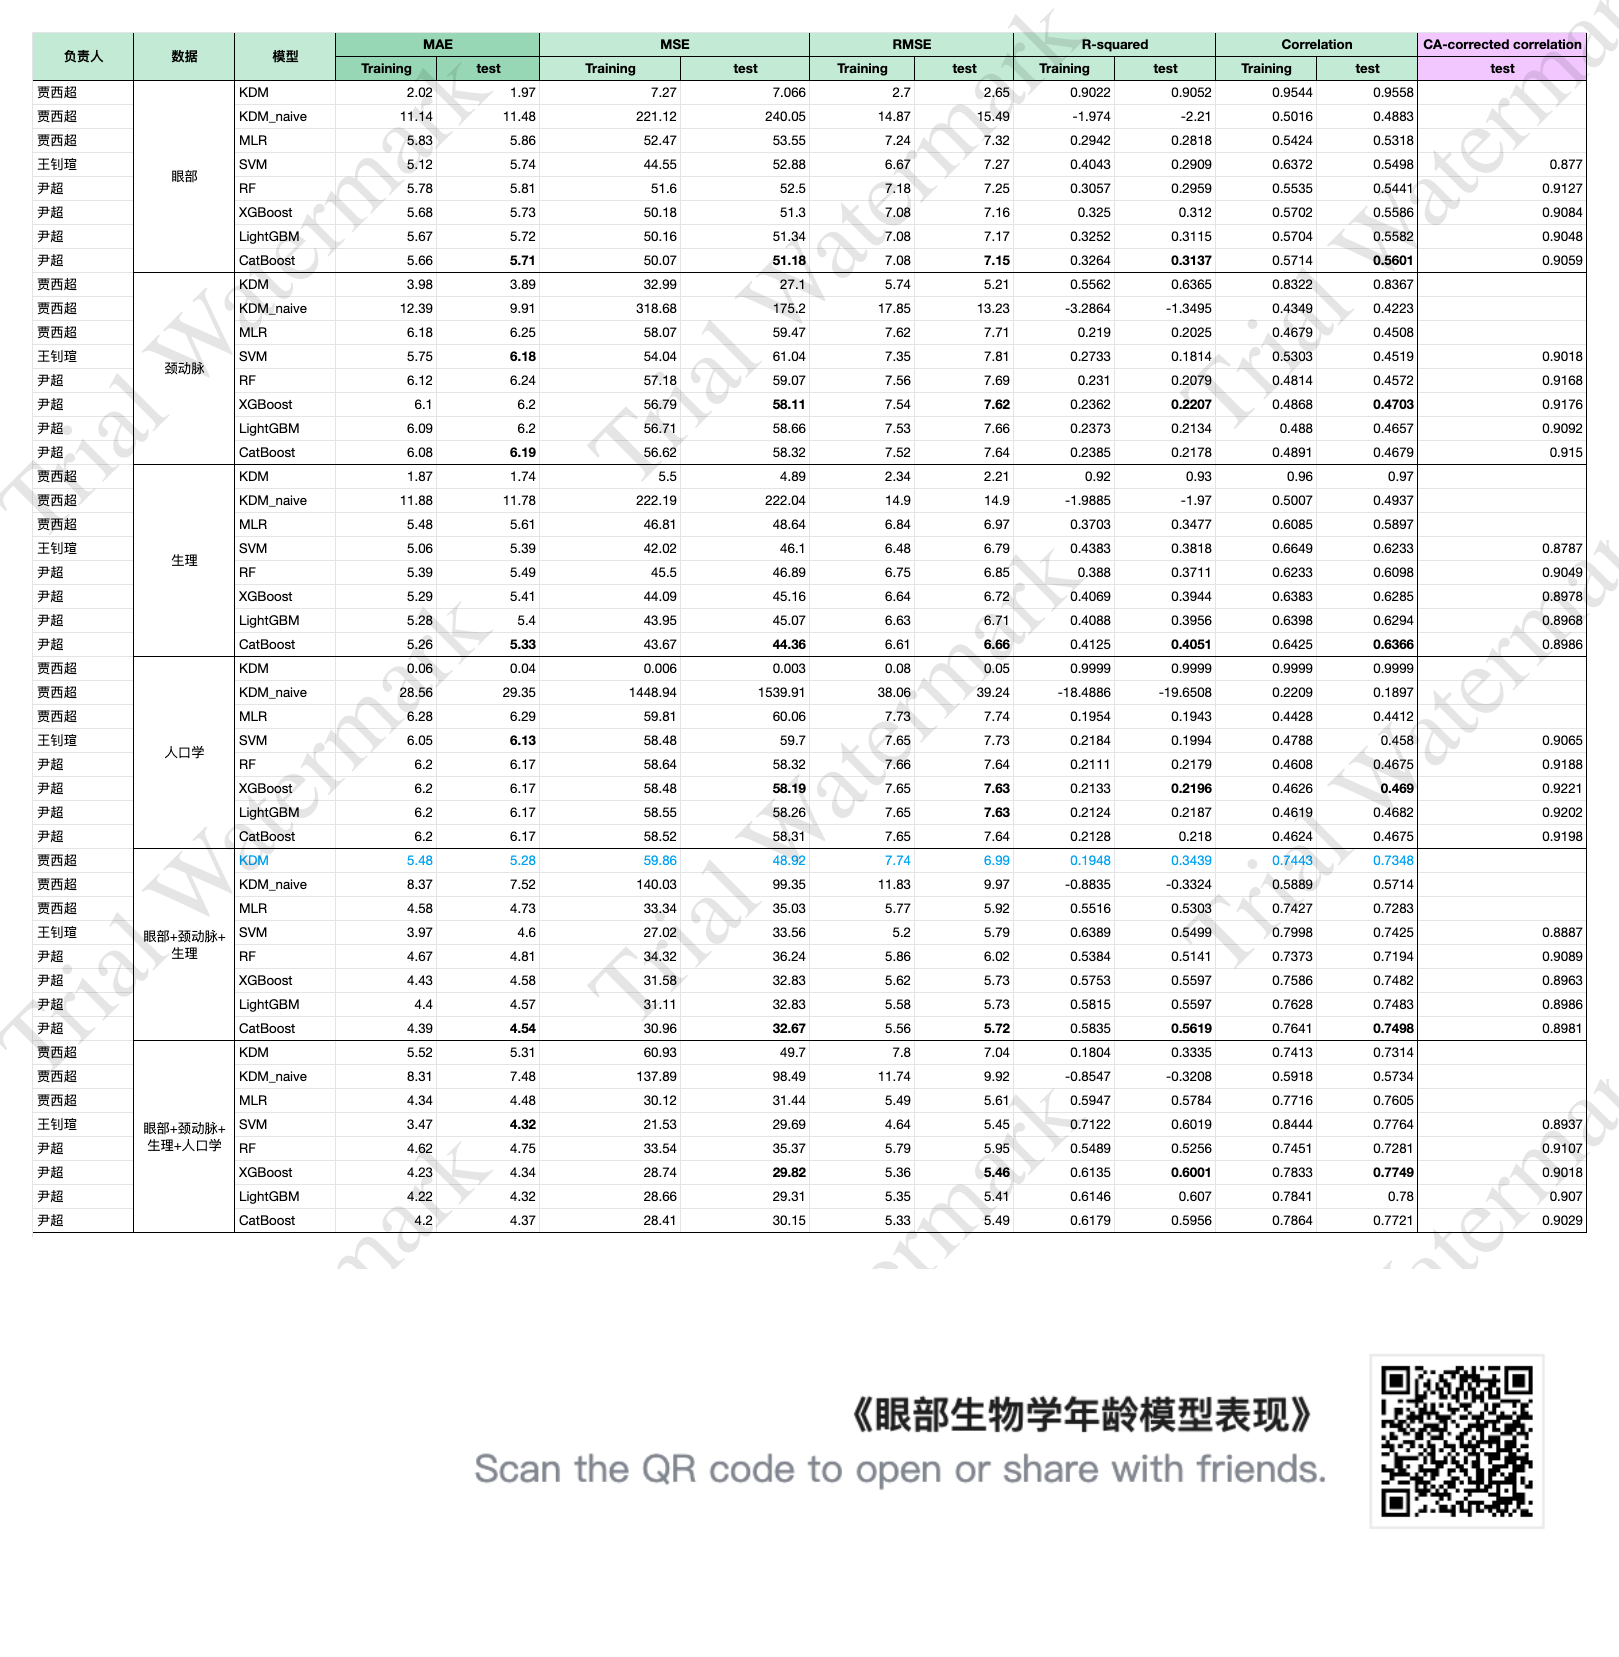
\includegraphics[width=1.0\textwidth]{assets/eye_table.png}
    \caption{所有模型结果对比}
    \label{fig:model_comparison}
\end{figure}

\chapter{工作总结}

\section{项目总结}
\section*{1. 数据分析与可视化(chart)}
本次数据分析工作主要通过可视化手段,对数据集中的疾病患病率和样本分布情况进行了探索。

\begin{itemize}
    \item \textbf{数据可视化:} 使用 Python 脚本(如 \texttt{disease\_groups\_histogram.py})绘制了多种直方图,以直观展示眼科疾病和其他疾病的患病率,以及在不同筛选条件下样本数量的分布。
    \item \textbf{结果呈现:} 最终产出了四张关键的可视化图表(\texttt{eye\_diseases\_bar.png}, \texttt{other\_diseases\_bar.png}, \texttt{exclude\_max\_histogram\_ultra\_high.png}, \texttt{max\_vs\_others\_histogram\_ultra\_high.png}),清晰地呈现了数据概况。
\end{itemize}


\subsection*{2. 原始数据修正(pre\_mod)}
\begin{itemize}
    \item \textbf{目的:} 确保原始 tsv 文件的格式统一和数据可用性。
    \item \textbf{执行:}
    \begin{itemize}
        \item 利用 \texttt{realign\_headers.py} 脚本为数据添加了 \texttt{samples} 列标题,保证了列的对齐。
        \item 通过 \texttt{convert\_yes\_to\_1.py} 和 \texttt{convert\_no\_to\_0.py} 脚本,将数据中的“yes”和“no”标记统一转换为1和0,为后续的数值计算做好了准备。
    \end{itemize}
\end{itemize}

\subsection*{3. 数据预处理(backup)}
\begin{itemize}
    \item \textbf{目的:} 对数据进行清洗、筛选和划分,以构建高质量的训练集和测试集。
    \item \textbf{执行:}
    \begin{itemize}
        \item \textbf{数据筛选:} 剔除了无疾病诊断信息的个体,并根据疾病类型(眼病、其他疾病)将样本划分为训练集和测试集。
        \item \textbf{数据划分:} 使用 \texttt{split\_train\_test.py} 脚本,按80\%训练集、20\%测试集的比例随机划分了数据集。
        \item \textbf{缺失值处理:}
        \begin{itemize}
            \item 可视化并剔除了缺失率超过50\%的字段。
            \item 对特定字段(如 \texttt{bmi}、\texttt{standing\_height} 等)应用了自定义的填充规则,并对其他缺失值进行了均值填充。
        \end{itemize}
        \item \textbf{特征选择:} 根据不同分析目的,筛选出了眼科、颈动脉、生理代谢、人口学以及所有字段组合,为后续模型训练提供不同维度的数据集。
    \end{itemize}
\end{itemize}

\subsection*{4. ICD10数据预处理(ICD10)}
\begin{itemize}
    \item \textbf{目的:} 将 ICD10 数据与原始 CKB 数据进行整合,剔除有病的个体。
    \item \textbf{执行:}
    \begin{itemize}
        \item 使用 \texttt{icd10.py} 脚本,将 ICD10 数据中的“yes”和“no”标记转换为1和0。
        \item 通过 \texttt{merge\_files.py} 脚本,将处理后的 ICD10 数据与预处理后的 CKB 数据进行合并,生成了包含更多疾病信息的综合数据集。
        \item 重复了数据预处理的步骤(剔除无诊断信息个体、划分训练测试集、剔除眼病患者等),确保合并后的数据集质量。
    \end{itemize}
\end{itemize}

\subsection*{5. 模型训练和测试(train\_test)}
\begin{itemize}
    \item \textbf{目的:} 在不同数据集上训练多种机器学习模型,并评估其预测生物学年龄的性能。
    \item \textbf{执行:}
    \begin{itemize}
        \item \textbf{模型选择:} 采用了 XGBoost、LightGBM、CatBoost 和 RandomForest 四种主流的决策树类算法。
        \item \textbf{训练与验证:} 在训练集上进行五折交叉验证,以平均绝对误差(MAE)为指标,寻找每个模型的最佳超参数。
        \item \textbf{性能评估:} 在独立的测试集上,评估了每种模型在不同数据组合(如 \texttt{all}, \texttt{artery}, \texttt{eye}, \texttt{ren} 等)下的预测性能。
    \end{itemize}
\end{itemize}

\subsection*{6.多模态模型的训练(multi\_modal)}
\begin{itemize}
    \item \textbf{目的:} 通过多模态数据融合,提高生物学年龄预测的准确性。
    \item \textbf{执行:}
    \begin{itemize}
        \item 采用了不同的融合策略,包括中期融合和晚期融合。
        \item 在每种融合策略下,使用相同的模型架构进行训练和评估。
    \end{itemize}
\end{itemize}

\subsection*{主要成果}
\begin{itemize}
    \item 成功构建了完整的数据处理和模型训练流程。
    \item 生成了详尽的模型性能对比报告,为后续研究提供了坚实的数据基础。
    \item 验证了不同数据维度对生物学年龄预测模型性能的影响。
\end{itemize}

\section{个人总结}
在本项目中,我深入参与了数据分析、超参数调优、模型训练等多个环节。

在师兄们的指导下,我逐渐掌握了项目的整体流程和各个环节的关键要点,提升了自己的技术能力和项目管理能力。

也懂得了不能过于依赖AI工具,仍需保持对数据和模型的深入理解。    

对于项目的每个环节,我都进行了详细的记录和总结,以便在未来的工作中能够更好地复用这些经验。

在总结工作时,我发现了项目仍有很多可优化的地方,例如步骤过分详细导致代码和数据tsv文件过多,可以进行步骤的融合,减少不必要的中间文件,节省内存。

在华大基因的一个月时间,收获良多,感谢师兄们的指导和帮助。


\chapter{AI工具相关}

\section{论文阅读}
这里非常推荐使用豆包进行论文阅读,可以直接上传论文的PDF文件进行阅读,随时提问。

\section{代码辅助}

我使用了多种AI工具来辅助代码编写和调试工作,例如:

GitHub Copilot , Cursor等第三方应用,调用了Claude Sonnet 3.7/4.0/4.1等模型。

一个较为明显的问题是AI工具在处理复杂逻辑时仍然存在局限性,有时无法完全理解开发者的意图,导致代码逻辑混乱或是结构混乱。(李祖琦师兄指出我用AI生成的代码有诸多问题)

这警示我们在使用AI工具时,必须保持对代码的高度关注和审查,不能完全依赖于AI的判断。

\section{问题解答}

对于一些术语和概念,我会使用Gemini 2.5 Flash , Grok 4 , ChatGPT 4o/5 进行解答。

%表格三线表:

% \begin{table}[H]
%    \centering
%    \caption{\textbf{符号含义与约定}}
%    \label{tab:waterpump}
%    \begin{tabular}{ccccc}
%    \toprule
%    符号 & 符号含义& 单位\\
%    \midrule
%    符号1& 含义1& 单位1\\
%    符号2& 含义2& 单位2\\
%    符号3& 含义3& 单位3\\
%    符号4& 含义4& 单位4\\
%    \bottomrule
%    \end{tabular}
% \end{table}








% ----------------------------------------------------------- %
% >> ---------------------- 参考文献 ---------------------- << %
% \nocite{*}
% \bibliography{re}
% \thispagestyle{fancy} 
% \addcontentsline{toc}{chapter}{参考文献}
%这里要用到 bibtex,使用xelatex->bibtex->xelatex->xelatex编译链
%同时要把re.bib文件放在同一目录下
%下面是re.bib文件的内容
% @book{knuth1984texbook,
%   author    = {Donald E. Knuth},
%   title     = {The TeXbook},
%   year      = {1984},
%   publisher = {Addison-Wesley},
% }

% @article{lamport1994latex,
%   author  = {Leslie Lamport},
%   title   = {LaTeX: A Document Preparation System},
%   journal = {Addison-Wesley},
%   year    = {1994},
% }

% @inproceedings{goossens1993latex,
%   author    = {Michel Goossens and Frank Mittelbach and Alexander Samarin},
%   title     = {The LaTeX Companion},
%   booktitle = {Addison-Wesley Series on Tools and Techniques for Computer Typesetting},
%   year      = {1993},
% }

% @misc{wikibibtex,
%   author       = {Wikipedia contributors},
%   title        = {BibTeX --- Wikipedia{,} The Free Encyclopedia},
%   year         = {2024},
%   url          = {https://en.wikipedia.org/wiki/BibTeX},
%   note         = {Accessed: 2025-04-15}
% }



% >> ---------------------- 参考文献 ---------------------- << %
% ----------------------------------------------------------- %



% ------------------------------------------------------------ %
% >> ------------------------ 附录 ------------------------ << %

% % 附录设置
% \newpage
% \appendix
% % chapter 标题自定义设置
% \titleformat{\chapter}[hang]{\normalfont\huge\bfseries\centering}{}{20pt}{}
% \titlespacing*{\chapter}{0pt}{-25pt}{8pt} % 控制上方空白的大小
% % section 标题自定义设置 
% \titleformat{\section}[hang]{\normalfont\centering\Large\bfseries}{\thesection}{8pt}{}




% 附录 A
% \chapter*{附录 A. 中英文对照表}\addcontentsline{toc}{chapter}{附录 A. 中英文对照表}   
% \thispagestyle{fancy} 
% \setcounter{section}{0}   
% \renewcommand\thesection{A.\arabic{section}}   
% \renewcommand{\thefigure}{A.\arabic{figure}} 
% \renewcommand{\thetable}{A.\arabic{table}}

% \section{中英文对照表}
% \begin{multicols}{2}  

%    \begin{table}[H]\centering
%    \caption{\textbf{中英文对照表}}
%    \begin{tabular}{cccccccc}\toprule
%        English & 中文 \\
%        \midrule
%        voltage            & 电压 \\
%        current            & 电流 \\
%        power              & 功率 \\
%        resistance         & 电阻 \\
%        conductance        & 电导 \\
%        inductance         & 电感 \\
%        capacitance        & 电容 \\
%        frequency          & 频率 \\
%        circuit            & 电路 \\
%        circuit element    & 电流元件 \\
%        signal             & 信号 \\
%        circuit analysis   & 电路分析 \\
%        circuit synthesis  & 电路综合 \\
%        circuit design     & 电路设计 \\
%        circuit topology   & 电路拓扑 \\
%        \bottomrule
%    \end{tabular}
%    \end{table}
    
%    \begin{table}[H]\centering
%        \caption{\textbf{中英文对照表}}
%        \begin{tabular}{cccccccc}\toprule
%            English & 中文 \\
%            \midrule
%            voltage            & 电压 \\
%            current            & 电流 \\
%            power              & 功率 \\
%            resistance         & 电阻 \\
%            conductance        & 电导 \\
%            inductance         & 电感 \\
%            capacitance        & 电容 \\
%            frequency          & 频率 \\
%            circuit            & 电路 \\
%            circuit element    & 电流元件 \\
%            signal             & 信号 \\
%            circuit analysis   & 电路分析 \\
%            circuit synthesis  & 电路综合 \\
%            circuit design     & 电路设计 \\
%            circuit topology   & 电路拓扑 \\
%            \bottomrule
%        \end{tabular}
%    \end{table}
% \end{multicols} 
    
% \section{支撑材料列表} 

% \begin{center}
%  这里插入一张图片(类似思维导图那种)
% \end{center}


% % 附录 B
% \chapter*{附录 B. 代码}\addcontentsline{toc}{chapter}{附录 B. 代码}   
% \thispagestyle{fancy} 
% \setcounter{section}{0}   
% \renewcommand\thesection{B.\arabic{section}}   
% \renewcommand{\thefigure}{B.\arabic{figure}} 
% \renewcommand{\thetable}{B.\arabic{table}}

% 注意:listing环境中手动输入的代码需要顶格写




% >> ------------------------ 附录 ------------------------ << %
% ------------------------------------------------------------ %

\end{document}

% VScode 常用快捷键:

% Ctrl + R:                 打开最近的文件夹
% F2:                       变量重命名
% Ctrl + Enter:             行中换行
% Alt + up/down:            上下移行
% 鼠标中键 + 移动:           快速多光标
% Shift + Alt + up/down:    上下复制
% Ctrl + left/right:        左右跳单词
% Ctrl + Backspace/Delete:  左右删单词    
% Shift + Delete:           删除此行
% Ctrl + J:                 打开 VScode 下栏(输出栏)
% Ctrl + B:                 打开 VScode 左栏(目录栏)
% Ctrl + `:                 打开 VScode 终端栏
% Ctrl + 0:                 定位文件
% Ctrl + Tab:               切换已打开的文件(切标签)
% Ctrl + Shift + P:         打开全局命令(设置)

% Latex 常用快捷键

% Ctrl + Alt + J:           由代码定位到PDF
% 


% Git提交规范:
% update: Linear Algebra 2 notes
% add: Linear Algebra 2 notes
% import: Linear Algebra 2 notes
% delete: Linear Algebra 2 notes
